\documentclass{standalone}

\usepackage{amssymb}
\usepackage{amsthm}
\usepackage{amsmath}


\usepackage{tikz}
\usetikzlibrary{shapes,backgrounds,calc,patterns}
\usepackage{venndiagram}


\begin{document}

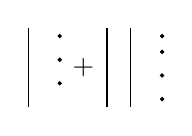
\begin{tikzpicture}
	\draw (0,0) -- (0,1);
	\draw[fill] (.4,.3) circle (.02);
	\draw[fill] (.4,.6) circle (.02);
	\draw[fill] (.4,.9) circle (.02);
	
	\node at (.7,.5) {\(+\)};
	
	\draw (1,0) -- (1,1);
	\draw (1.3,0) -- (1.3,1);
	\draw[fill] (1.7,.1) circle (.02);	
	\draw[fill] (1.7,.4) circle (.02);
	\draw[fill] (1.7,.7) circle (.02);
	\draw[fill] (1.7,.9) circle (.02);
\end{tikzpicture}
\end{document}